% Options for packages loaded elsewhere
\PassOptionsToPackage{unicode}{hyperref}
\PassOptionsToPackage{hyphens}{url}
%
\documentclass[
]{book}
\usepackage{lmodern}
\usepackage{amssymb,amsmath}
\usepackage{ifxetex,ifluatex}
\ifnum 0\ifxetex 1\fi\ifluatex 1\fi=0 % if pdftex
  \usepackage[T1]{fontenc}
  \usepackage[utf8]{inputenc}
  \usepackage{textcomp} % provide euro and other symbols
\else % if luatex or xetex
  \usepackage{unicode-math}
  \defaultfontfeatures{Scale=MatchLowercase}
  \defaultfontfeatures[\rmfamily]{Ligatures=TeX,Scale=1}
\fi
% Use upquote if available, for straight quotes in verbatim environments
\IfFileExists{upquote.sty}{\usepackage{upquote}}{}
\IfFileExists{microtype.sty}{% use microtype if available
  \usepackage[]{microtype}
  \UseMicrotypeSet[protrusion]{basicmath} % disable protrusion for tt fonts
}{}
\makeatletter
\@ifundefined{KOMAClassName}{% if non-KOMA class
  \IfFileExists{parskip.sty}{%
    \usepackage{parskip}
  }{% else
    \setlength{\parindent}{0pt}
    \setlength{\parskip}{6pt plus 2pt minus 1pt}}
}{% if KOMA class
  \KOMAoptions{parskip=half}}
\makeatother
\usepackage{xcolor}
\IfFileExists{xurl.sty}{\usepackage{xurl}}{} % add URL line breaks if available
\IfFileExists{bookmark.sty}{\usepackage{bookmark}}{\usepackage{hyperref}}
\hypersetup{
  pdftitle={Photochemistry and Photophysics Workshops},
  pdfauthor={Fiona Dickinson},
  hidelinks,
  pdfcreator={LaTeX via pandoc}}
\urlstyle{same} % disable monospaced font for URLs
\usepackage{longtable,booktabs}
% Correct order of tables after \paragraph or \subparagraph
\usepackage{etoolbox}
\makeatletter
\patchcmd\longtable{\par}{\if@noskipsec\mbox{}\fi\par}{}{}
\makeatother
% Allow footnotes in longtable head/foot
\IfFileExists{footnotehyper.sty}{\usepackage{footnotehyper}}{\usepackage{footnote}}
\makesavenoteenv{longtable}
\usepackage{graphicx}
\makeatletter
\def\maxwidth{\ifdim\Gin@nat@width>\linewidth\linewidth\else\Gin@nat@width\fi}
\def\maxheight{\ifdim\Gin@nat@height>\textheight\textheight\else\Gin@nat@height\fi}
\makeatother
% Scale images if necessary, so that they will not overflow the page
% margins by default, and it is still possible to overwrite the defaults
% using explicit options in \includegraphics[width, height, ...]{}
\setkeys{Gin}{width=\maxwidth,height=\maxheight,keepaspectratio}
% Set default figure placement to htbp
\makeatletter
\def\fps@figure{htbp}
\makeatother
\setlength{\emergencystretch}{3em} % prevent overfull lines
\providecommand{\tightlist}{%
  \setlength{\itemsep}{0pt}\setlength{\parskip}{0pt}}
\setcounter{secnumdepth}{5}
\usepackage{booktabs}
\usepackage{amsthm}
\makeatletter
\def\thm@space@setup{%
  \thm@preskip=8pt plus 2pt minus 4pt
  \thm@postskip=\thm@preskip
}
\makeatother
\ifluatex
  \usepackage{selnolig}  % disable illegal ligatures
\fi
\usepackage[]{natbib}
\bibliographystyle{apalike}

\title{Photochemistry and Photophysics Workshops}
\author{Fiona Dickinson}
\date{2020-09-25}

\begin{document}
\maketitle

{
\setcounter{tocdepth}{1}
\tableofcontents
}
\hypertarget{welcome}{%
\chapter*{Welcome}\label{welcome}}
\addcontentsline{toc}{chapter}{Welcome}

The notes have been prepared in a package called BookDown for RStudio so that the equations are accessible to screen readers. However, by providing the notes as a .html webpage I can also embed short videos to further describe some of the topics. Further you can download the questions (and later the answers, top left of the screen) in a format that suits you (either pdf or epub) to view offline, or change the way this document appears for ease of reading.

\hypertarget{ch:WorkIntro}{%
\chapter{Workshops for Photochemistry \& Photophysics}\label{ch:WorkIntro}}

The course will use a question first approach and we will learn the material by answering the questions. The questions will be shared here in an accessible format, and this page will be updated weekly.

\hypertarget{version-history}{%
\section*{Version history}\label{version-history}}
\addcontentsline{toc}{section}{Version history}

The initial commit of this book is dated 25th September 2020.

\hypertarget{ch:Workshop1}{%
\chapter{Workshop Questions for Week 1}\label{ch:Workshop1}}

\hypertarget{sec:BeerLambert}{%
\section{Short mathematical question - Beer Lambert law}\label{sec:BeerLambert}}

\begin{itemize}
\tightlist
\item
  How far can monochromatic 489 nm light travel through a 0.100 M solution of fluorescein with an extinction coefficient at 489 nm of 92000 M\textsuperscript{−1} cm\textsuperscript{−1} before 90 \% of it is absorbed?
  \emph{(I will use MCQs and UniDoodle to ask this in class)}
\end{itemize}

\hypertarget{sec:MolarExtinction}{%
\section{Short conceptual question - molar extinction coefficient}\label{sec:MolarExtinction}}

\begin{itemize}
\tightlist
\item
  Modify the molecule in figure \ref{fig:bpy} to increase the molar extinction coefficient (do not worry about what may happen to wavelength).
\end{itemize}

\begin{figure}

{\centering 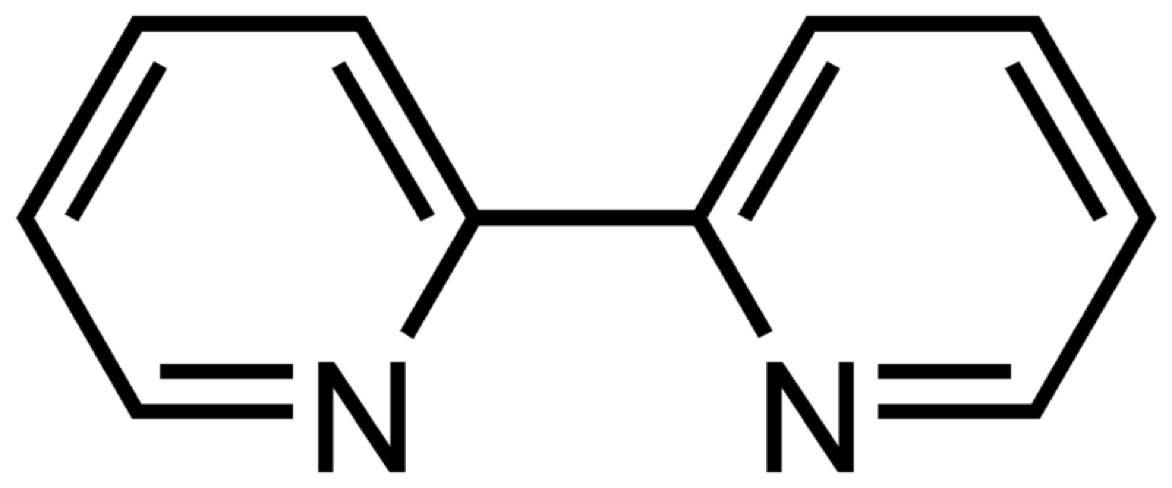
\includegraphics[width=0.7\linewidth]{images/bpy} 

}

\caption{The structures of the organic dye methylene blue (left), potassium permanganate (centre) and copper hexa-aqua (right).}\label{fig:bpy}
\end{figure}

\emph{(I will use UniDoodle's drawing feature to ask this in class)}

\hypertarget{sec:intensity}{%
\section{Short conceptual question - intensity of colour}\label{sec:intensity}}

\begin{itemize}
\tightlist
\item
  What factors influence the `intensity of colour' of the following solutions?
\end{itemize}

\begin{figure}

{\centering 
\includegraphics[width=0.7\linewidth]{images/molarextquestion} 

}

\caption{The structures of the organic dye methylene blue (left), potassium permanganate (centre) and copper hexa-aqua (right).}\label{fig:molarextstructures}
\end{figure}

\begin{figure}

{\centering 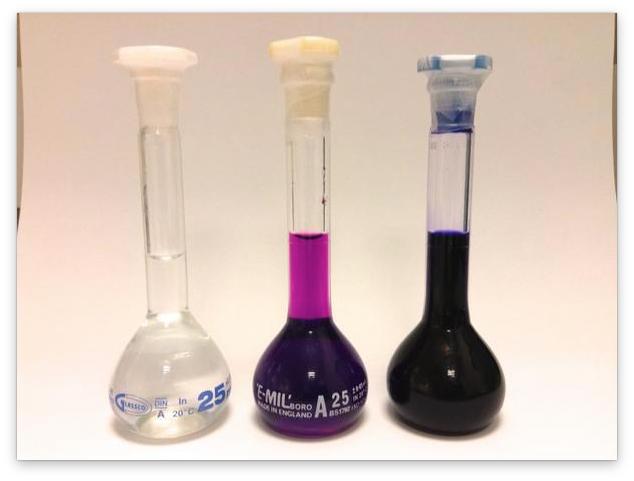
\includegraphics[width=0.7\linewidth]{images/Molar_extinction_coefficients} 

}

\caption{1 mM solutions of the organic dye methylene blue (right), potassium permanganate (centre) and copper hexa-aqua (right).}\label{fig:molarextsolutions}
\end{figure}

\emph{(This will be a discussion question - please feel free to raise a hand or write comments in the zoom chat)}

\hypertarget{sec:linewidth}{%
\section{Short conceptual question - line width}\label{sec:linewidth}}

\begin{itemize}
\tightlist
\item
  Why are some spectra very broad (figure \ref{fig:molecular}), whereas others have sharp peaks (figure \ref{fig:atomic})?
\end{itemize}

You will need to look at the x-scale to truley note the difference in the width of these emission spectra.

\begin{figure}

{\centering 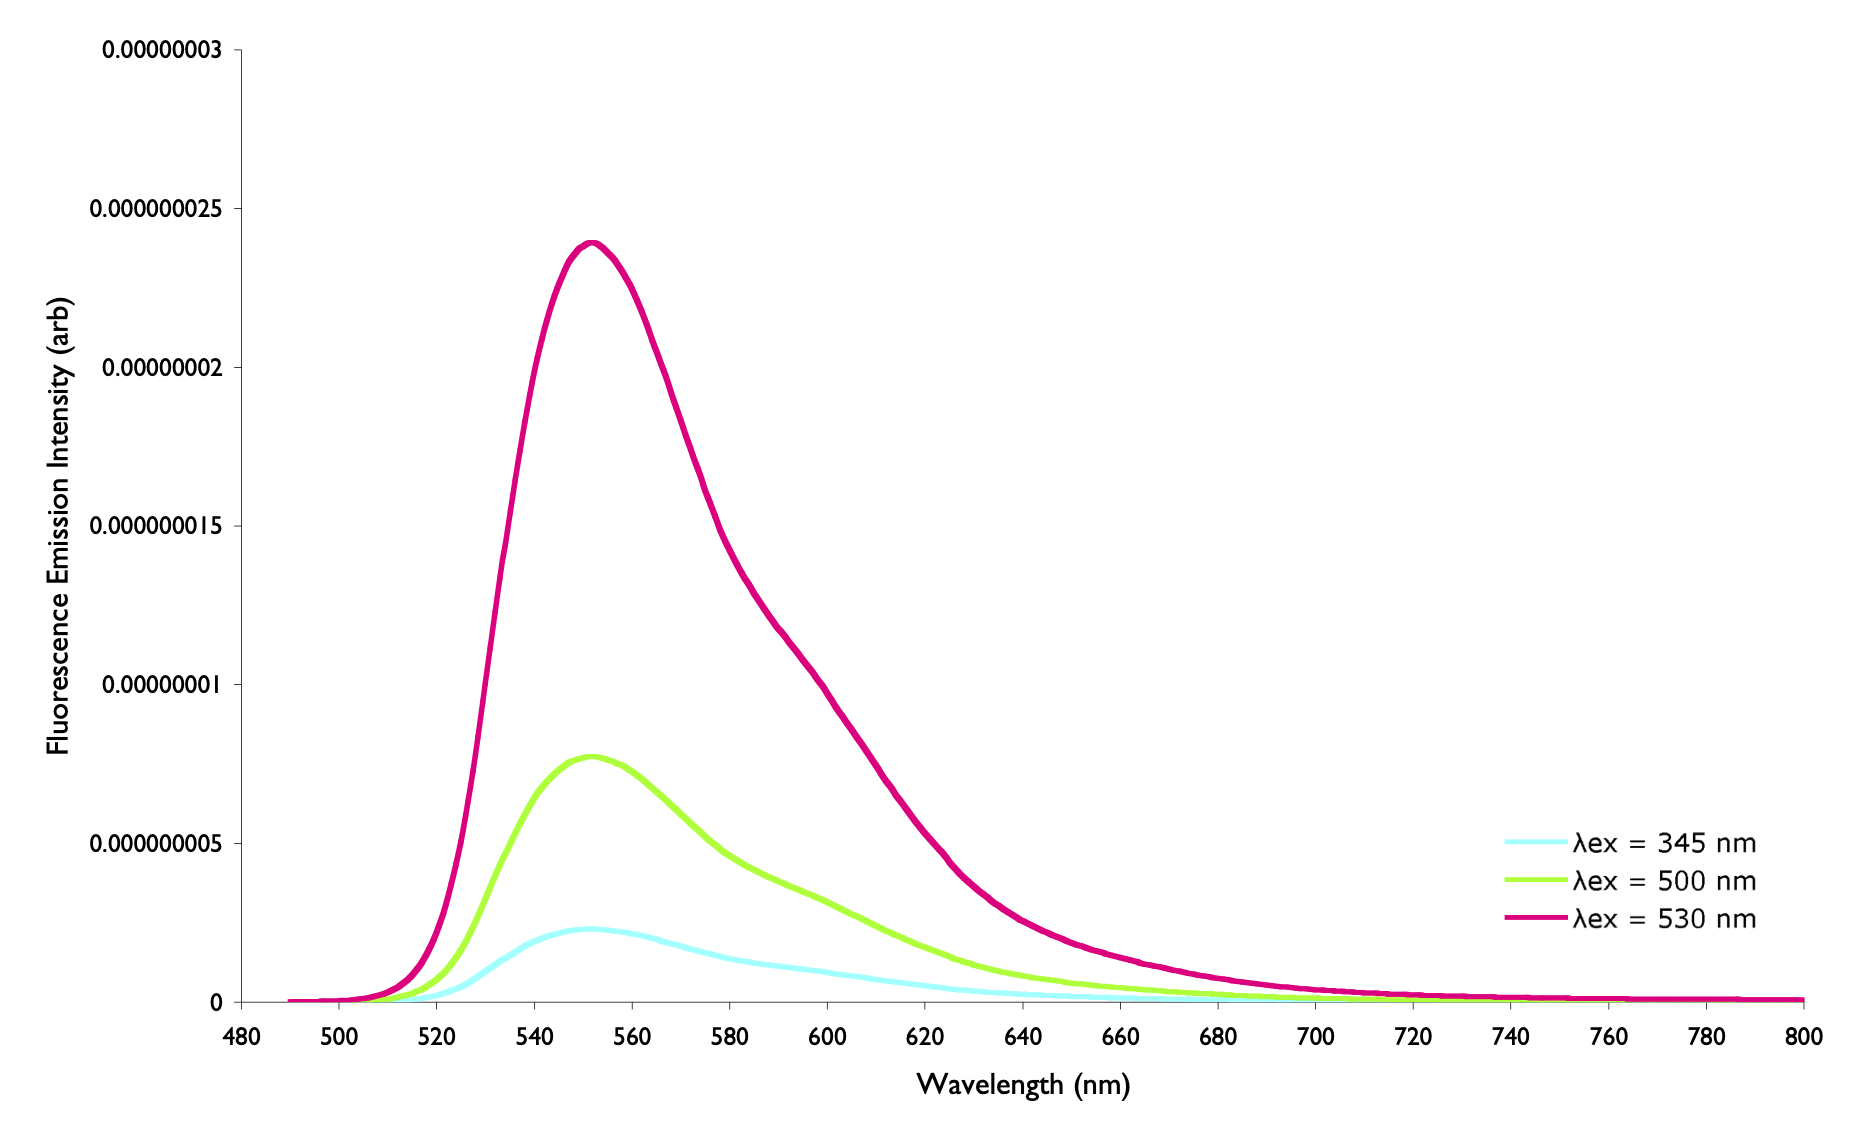
\includegraphics[width=0.7\linewidth]{images/rhodamine6G} 

}

\caption{The emission spectrum of rhodamine 6G}\label{fig:molecular}
\end{figure}

\begin{figure}

{\centering 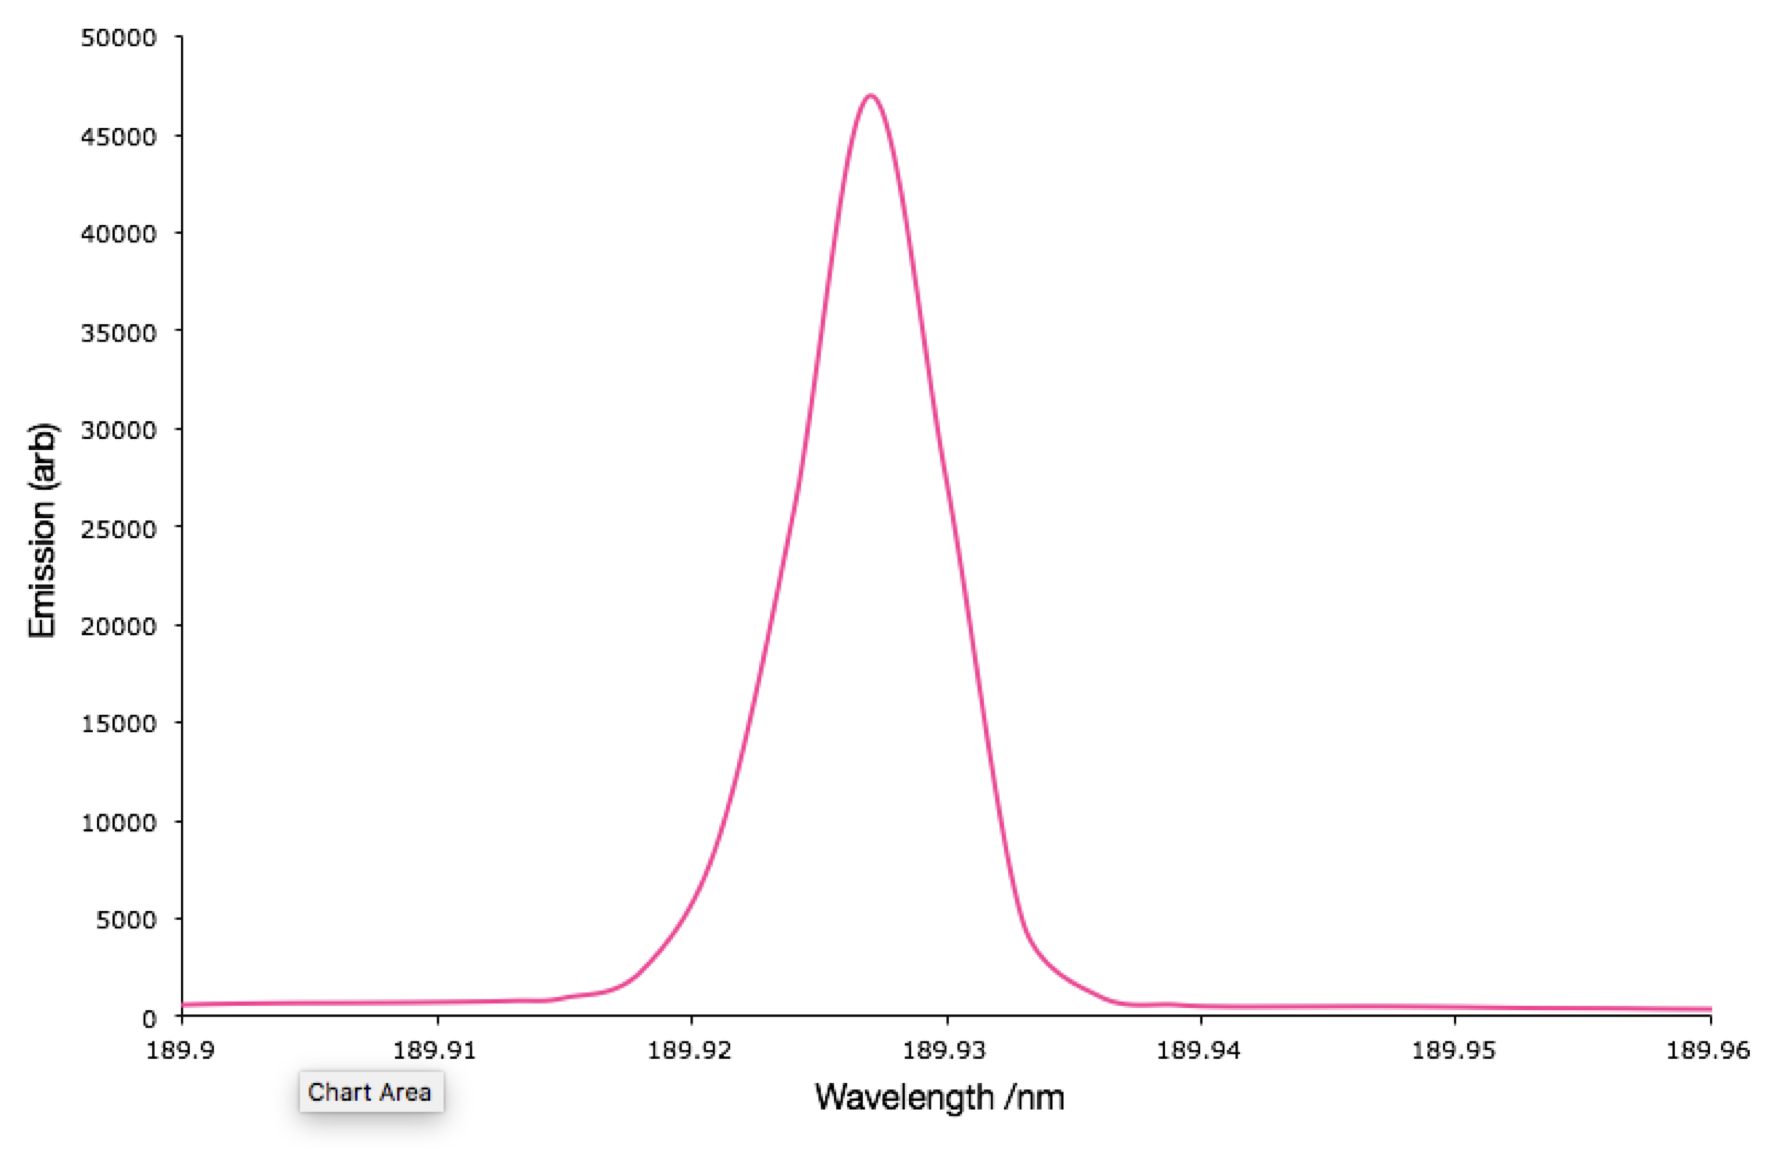
\includegraphics[width=0.7\linewidth]{images/atomic_emission_spectrum} 

}

\caption{The emission spectrum of Sn(II)}\label{fig:atomic}
\end{figure}

\emph{(This will be a discussion question - please feel free to raise a hand or write comments in the zoom chat)}

\hypertarget{sec:solvationabs}{%
\section{Short conceptual question - the effect of solvation on absorbance}\label{sec:solvationabs}}

\begin{figure}

{\centering 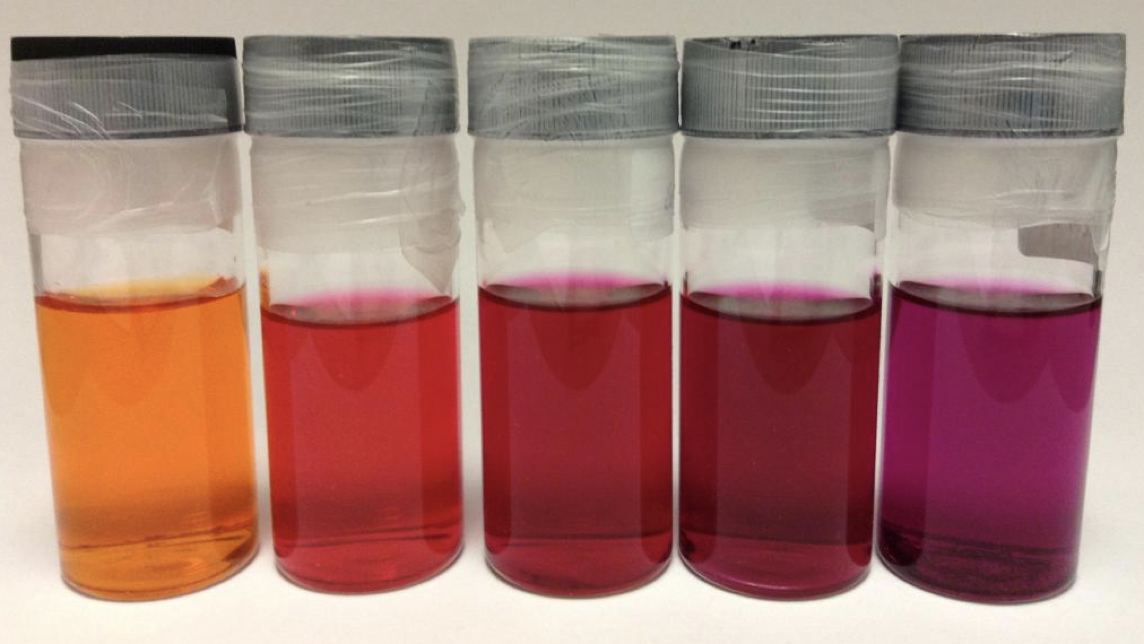
\includegraphics[width=0.7\linewidth]{images/ethidium} 

}

\caption{Ethidium bromide dissolved in from right; water(orange), methanol, ethanol, propanol and butanol(purple)}\label{fig:ethidium}
\end{figure}

\begin{itemize}
\tightlist
\item
  Why does the observed colour of ethidium bromide depend upon the solvent (figure \ref{fig:ethidium}))?
\end{itemize}

Think about the effect of solvation on the energy levels and why those energy levels matter! Remember that if light is transmitted through a solution that is the colour we observe\ldots{}

\emph{(This will be a discussion question - please feel free to raise a hand or write comments in the zoom chat)}

\hypertarget{sec:Azobenzene}{%
\section{Extended question - Azobenzene}\label{sec:Azobenzene}}

Azobenzene undergoes the following cis-trans isomerisation, the isomerisation occurs in the ps timescale.

\begin{figure}

{\centering 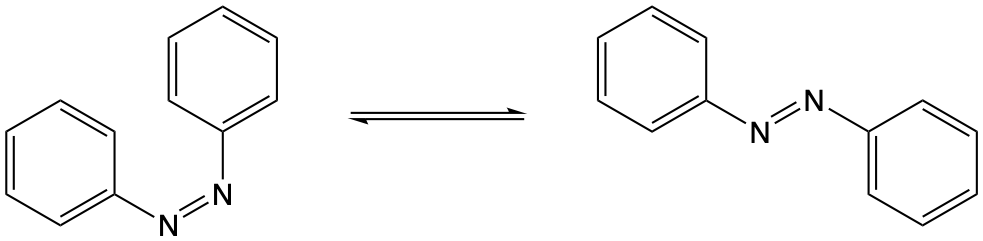
\includegraphics[width=0.7\linewidth]{images/cistransazobenzene} 

}

\caption{The cis-trans isomerisation of azobenzene}\label{fig:cistransazobenzene}
\end{figure}

\begin{itemize}
\item
  Why would you expect the absorption spectrum of each isomer to be different?
\item
  Suggest why the trans conformation is more stable than the cis isomer.
\item
  Use the following data to predict the proportion of each isomer under 360 nm excitation.
  Table: \label{tab:azobenzneabs} The molar extinction coefficient of the two isomers of azobenzene.
\end{itemize}

\begin{longtable}[]{@{}lll@{}}
\toprule
& ε\textsubscript{360} / M\textsuperscript{−1} cm\textsuperscript{−1} & ε\textsubscript{460} / M\textsuperscript{−1} cm\textsuperscript{−1}\tabularnewline
\midrule
\endhead
trans-azobenzene & 22000 & 4500\tabularnewline
cis-azobenzene & 2100 & 5500\tabularnewline
\bottomrule
\end{longtable}

\begin{itemize}
\item
  Would there be more or less trans azobenzene at 460 nm? Justify your answer.
\item
  It has been suggested the 360 nm absorption is an S\textsubscript{0} → S\textsubscript{2} absorption, and the 460 nm band is an S\textsubscript{0} → S\textsubscript{1} absorption. Suggest which energy levels are involved for each of the two transitions and compare it to stilbene which has a similar structure, but the cis and trans absorptions are 280 \& 295 nm respectively.
\end{itemize}

\begin{figure}

{\centering 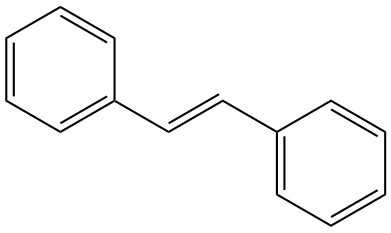
\includegraphics[width=0.7\linewidth]{images/stilbene} 

}

\caption{The  structure of stilbene}\label{fig:stilbene}
\end{figure}

\emph{(This will be a discussion question - please feel free to raise a hand or write comments in the zoom chat. I don't expect to finish this question but hope to get far enough through that a good attempt can be made at home after the LOIL)}

  \bibliography{book.bib,packages.bib}

\end{document}
